\documentclass[../../Main/Apputni Fisica.tex]{subfiles}
\begin{document}
In termodinamica, lo stato di un sistema è descritto da variabili di stato, quali pressione, volume, ecc.
Si ha però che se un sistema è in equilibrio termico, è possibile specificare lo stato dello stesso.
\\ \\
Si consideri un cilindro contente gas, munito di un pistone mobile.
Se \(A\) è l'area di sezione del pistone, sul gas si imporra una forza \(\vb{F} = \vb{P}A\).
Abbassando, quasi staticamente, il pistone di un certo tratto \({\dd \vb{s}} = {\dd y}\), il lavoro sul gas è
\[
    {\dd \vb{W}} = \va{F} \cdot {\dd \va{s}} = - \vb{P}A {\dd y}
\]
ma \(A {\dd y} = \Delta V\), segue
\[
    {\dd \vb{W}} = - \vb{P} \Delta V
\]
%
Integrando da \(V_{i} \text{a} V_{f}\), segue quindi
\begin{equation}\label{eq:9}
    \vb{W} = \int{V_{i}}{V_{f}}{-\vb{P}}{V}
\end{equation}
%
Se \(\vb{P} \text{e} V\) sono noti in ogni punto, allora lo stato del sistema è rappresentabile con il \textit{diagramma PV}.
\begin{Example*}
    Siano \(V_{i}\) il volume iniziale, \(V_{f}\) quella finale, e siano \(\vb{P_{i}}\) la pressione iniziale e \(\vb{P_{f}}\) quella finale,
    si riporti corrispondente il diagramma PV, stabilendo con \(f\) lo stato finale, e con \(i\) quello iniziale.

    \begin{figure}[!h]
        \centering
        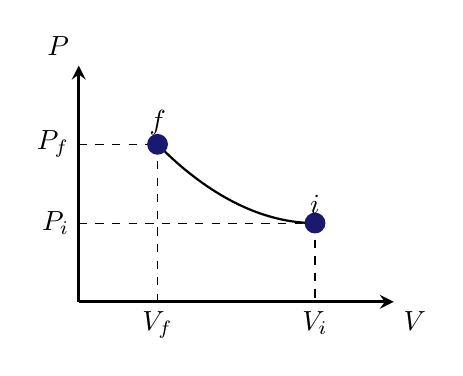
\begin{tikzpicture}[scale = 1, every node/.style={scale=1}]

            % Drawing axis
            \draw [-stealth, very thick] (0, 0) -- (0, 3);
            \node [anchor = south east] at (0, 3) {\(\vb{P}\)};

            \draw [-stealth, very thick] (0, 0) -- (4, 0);
            \node [anchor = north west] at (4, 0) {\(V\)};

            % Pressure values
            \draw [dashed] (0, 1) -- (3, 1);
            \node [anchor = east] at (0, 1) {\(\vb{P_{i}}\)};

            \draw [dashed] (0, 2) -- (1, 2);
            \node [anchor = east] at (0, 2) {\(\vb{P_{f}}\)};

            % Volume Values
            \draw [dashed] (1, 2) -- (1, 0);
            \node [anchor = north] at (1, 0) {\(V_{f}\)};

            \draw [dashed] (3, 1) -- (3, 0);
            \node [anchor = north] at (3, 0) {\(V_{i}\)};

            % Thermodynamic transformation
            \draw [thick] (3, 1) parabola (1, 2);

            % State points
            \draw [fill = MidnightBlue, color = MidnightBlue] (3, 1) circle (0.125);
            \node [anchor = south] at (3, 1) {\(i\)};

            \draw [fill = MidnightBlue, color = MidnightBlue] (1, 2) circle (0.125);
            \node [anchor = south] at (1, 2) {\(f\)};
        \end{tikzpicture}
        \caption{Esempio di diagramma PV.}
        \label{fig:9}
    \end{figure}
\end{Example*}
\end{document}